\documentclass{beamer}				
\mode<presentation>
{
\usetheme{Warsaw}I
\setbeamercovered{transparent}
}
\usepackage[T1]{fontenc}
\usepackage[utf8]{inputenc}
\usepackage{graphicx}
\usepackage{polski}
\usepackage{times}

\usepackage{tikz}
\usetikzlibrary{shapes.geometric, arrows}
\tikzstyle{decision} = [diamond, draw, fill=yellow!20, minimum height=3em,
    text width=6em, text badly centered, node distance=3cm, inner sep=0pt]
\tikzstyle{block} = [rectangle, draw, fill=blue!20, 
    text width=8em, text centered, rounded corners, minimum height=3em]
\tikzstyle{scilab} = [circle, draw, fill=green!20, 
    text width=8em, text centered,  minimum height=2em]
\tikzstyle{cloud} = [draw, ellipse,fill=red!20, node distance=3cm,
    text width=8em, text centered, minimum height=4em]
\tikzstyle{line} = [draw, -latex']

\usepackage{xcolor}
\newcommand\crule[3][black]{\textcolor{#1}{\rule{#2}{#3}}}


\definecolor{grey}{HTML}{808080}
\definecolor{redrect}{HTML}{FE0000}

\author[Magdalena Jóźwiakowska, Mikołaj Buchwald]
{
Magdalena Jóźwiakowska
\and
Mikołaj Buchwald
}
\title[EEG ANN]
{"Wykrywanie artefaktów mrugania w sygnale EEG przy pomocy Sztucznych Sieci Neuronalnych"}
\subtitle
{Laboratorium Programowanie\\Sprawozdanie z projektu zaliczeniowego}



\begin{document}
%%%%%%%%%%%%%%%%%%%%%%%%%%%%%%%%%%%%%%%%%%%%%%%%%%%%
%%%%%%%%%%%%%%%%%%%%%%%%%%%%%%%%%%%%%%%%%%%%%%%%%%%%

\begin{frame}			%%%% SLAJD TYTUŁOWY
  \maketitle
\end{frame}


\begin{frame}
    \frametitle{Wprowadzenie}

    \begin{figure}
        \centering
        \only<1->{\includegraphics[scale=0.3]{eyes.png}}
    \end{figure}
    \begin{columns}
        \begin{column}{0.5\textwidth}
            \only<2->{\includegraphics[width=1\textwidth]{mwm.png}}
        \end{column}
        \begin{column}{0.5\textwidth}
            \only<3->{\includegraphics[scale=0.2]{ann.png}}
        \end{column}
    \end{columns}
\end{frame}

\begin{frame}	
    \frametitle{Materiały i metody}
    \framesubtitle{Software oraz hardware}
    \pause
    \begin{block}{Platforma}
        \pause
        \begin{itemize} [<+->]
            \item Linux Debian
        \end{itemize}
    \end{block}
    \begin{block}{EEG}
        \pause
        \begin{itemize} [<+->]
            \item MindWave Mobile firmy NeuroSky
            \item Częstotliwość próbkowania: 512 Hz
        \end{itemize}
    \end{block}
\end{frame}



\begin{frame}	
    \frametitle{Materiały i metody}
    \framesubtitle{Użyte języki programowania}
    \begin{block}{Python}
        \pause
        PsychoPy  \\ \pause
            \begin{itemize} [<+->]
                \item Eksperyment do zbierania danych do szkolenia Sieci
                \item Eksperyment do zbierania danych do kategoryzacji
            \end{itemize}
        \pause
        Python skrypty  \\ \pause
            \begin{itemize} [<+->]
                \item Dzielenie danych na zbiory próbek oraz paczek
                \item Ekstrakcja cech
                \item Generowanie wyników
                \item Generowanie danych do wykresów
            \end{itemize}
    \end{block}
\end{frame}

\begin{frame}	
    \frametitle{Materiały i metody}
    \framesubtitle{Użyte języki programowania}
    \pause
    \begin{block}{C}
        FANN (Fast Artificial Neural Network):  \\ \pause
            \begin{itemize} [<+->]
                \item Szkolenie Sieci	
                \item Kategoryzacja danych  				
            \end{itemize}
    \end{block}

\end{frame}

\begin{frame}	
    \frametitle{Materiały i metody}
    \framesubtitle{Dodatkowe skrypty}
    \pause

    \begin{block}{Scilab}
        \pause
        Generowanie wykresów
    \end{block}

    \pause

    \begin{block}{Bash}
        \pause
        Pomocniczo przy odpalaniu programów oraz skryptów
    \end{block}

    \pause

    \begin{block}{\LaTeX}
        \pause
        \begin{itemize} [<+->]
            \item Beamer prezentacja	
            \item Tex sprawozdanie
        \end{itemize}
    \end{block}
\end{frame}

\begin{frame}
    \frametitle{Materiały i metody}
    \framesubtitle{Schemat ilustrujący procedurę zbierania oraz przetrwarzania danych}

    \begin{figure}[H]
        \fontsize{8pt}{10pt}\selectfont
        \hspace*{-0.9cm} 
        \centering
        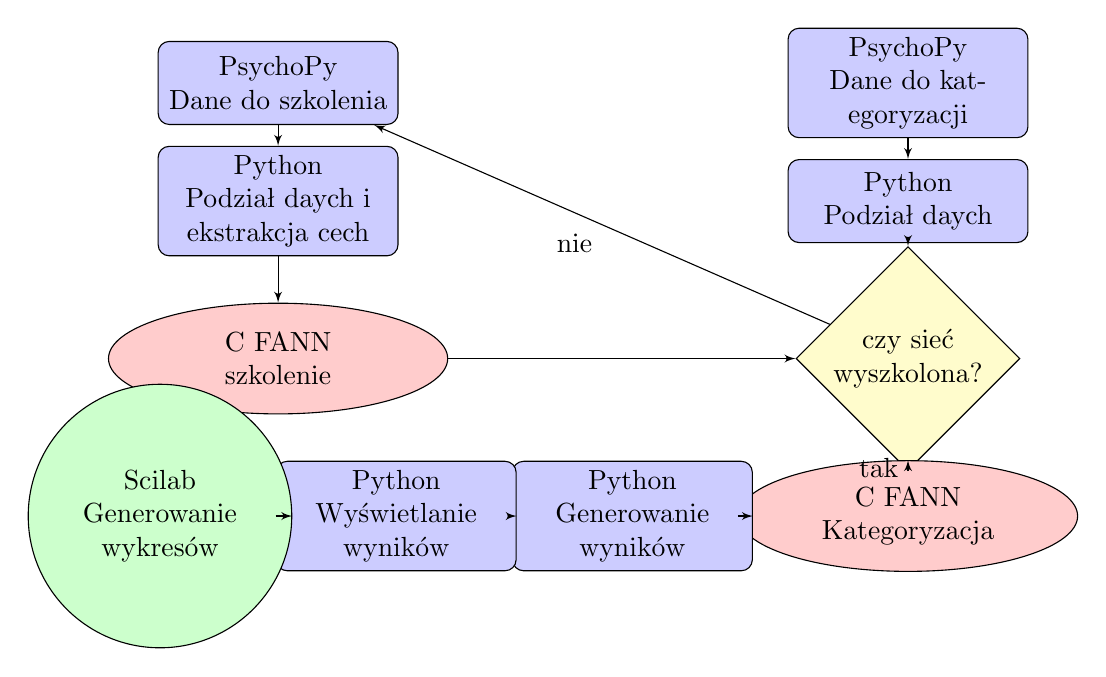
\begin{tikzpicture}[node distance = 2cm, auto]
            % Place nodes
            \node [block] (init) {PsychoPy \\ Dane do szkolenia};
            \node [block, below of=init, node distance=1.5cm] (extr) {Python \\Podział daych i ekstrakcja cech};
            \node [block, right of=init, node distance=8cm] (dane2){PsychoPy \\Dane do kategoryzacji};
            \node [block, below of=dane2, node distance=1.5cm] (split) {Python \\Podział daych};
            \node [cloud, below of=extr, node distance=2cm] (train) {C FANN \\szkolenie};
            \node [decision, below of=split, node distance=2cm] (decide) {czy sieć wyszkolona?};
            \node [cloud, below of=decide, node distance=2cm] (categ) {C FANN \\Kategoryzacja};
            \node [block, left of=categ, node distance=3.5cm] (plot) {Python \\Generowanie wyników};
            \node [block, left of=plot, node distance=3cm] (result) {Python \\Wyświetlanie wyników};
            \node [scilab, left of=result, node distance=3cm] (sci) {Scilab \\Generowanie wykresów};
            % Draw edges
            \path [line] (init) -- (extr);
            \path [line] (dane2) -- (split);
            \path [line] (extr) -- (train);
            \path [line] (split) -- (decide);
            \path [line] (train) -- (decide);
            \path [line] (decide) -- node [near start] {tak} (categ);
            \path [line] (decide) -- node {nie}(init);
            \path [line] (categ) -- (plot);
            \path [line] (plot) -- (result);
            \path [line] (result) -- (sci);
        \end{tikzpicture}
    \end{figure}
\end{frame}

\begin{frame}	
    \frametitle{Materiały i metody}
    \framesubtitle{Przebieg eksperymentu}
    \pause
    \begin{block}{Specyfikacja próby}
        \pause
        \begin{itemize} [<+->]
            \item Przebadano 3 osoby w wieku 20-22 lata
            \item Wszystkie one były studentami
        \end{itemize}
    \end{block}
\end{frame}

\begin{frame}	
    \frametitle{Materiały i metody}
    \framesubtitle{Przebieg eksperymentu}
    \pause
    \begin{block}{Instrukcje początkowe}
        \pause
        \begin{itemize} [<+->]
            \item Etap zbierania danych do szkolenia sieci:\\
                "Na środku ekranu pojawiać się będzie czerwony kwadrat. 
                Gdy pojawi się kwadrat mrugnij proszę jeden raz. 
                Nie wolno Ci mrugać w przypadku innym niż pojawienie się kwadratu." 
            \item Etap zbierania danych do kategoryzacji:\\
                "Na środku ekranu pojawiać się będzie czerwony kwadrat. 
                Gdy pojawi się kwadrat mrugaj tak długo jak długo widzisz kwadrat. 
                Staraj się proszę by mrugnięcia były jak najbardziej spontaniczne. 
                Mrugaj raz za razem nie robiąc przerw. 
                Nie wolno Ci mrugać w przypadku innym niż pojawienie się kwadratu." 
        \end{itemize}
    \end{block}
\end{frame}

\begin{frame}[plain]{}
    
\begin{tikzpicture}
        \hspace*{-1cm}
        \draw[fill=grey] (0,0) rectangle (16,10);
        \hspace*{1cm}
    \end{tikzpicture}
\end{frame}

\begin{frame}[plain]{}
    
\begin{tikzpicture}
        \hspace*{-1cm}
        \draw[fill=grey] (0,0) rectangle (16,10);
        \hspace*{1cm}
        \begin{scope}[xshift=2.7cm, yshift=2.8cm]
            \fill[redrect] (2,2) rectangle (3,3);
        \end{scope}
    \end{tikzpicture}
\end{frame}

\begin{frame}
\frametitle{Wyniki}
    \begin{table}[H]
        \caption {Wyniki wkaźników dla poszczególnych osób badanych}
        \begin{center}
            \hspace*{-0.5cm}
            \begin{tabular}{| p{2.5cm} || c | c | c || c |}
                \hline
                 & Osoba 001 & Osoba 002 & Osoba 003 & Razem \\
                \hline
                \hline
                Wskaźnik\_01 & 100\% & 100\% & 100\% & 100\% \\
                \hline
                Wskaźnik\_02 &   0\% &  71\% &  28\% &  33\% \\
                \hline
                Wskaźnik\_03 &   0\% &  71\% &  28\% &  33\% \\
                \hline
                \hline
                Ogólny wynik & 100\% &  29\% &  72\% &  67\% \\
                \hline
            \end{tabular}
        \end{center}
    \end{table}
\end{frame}

\begin{frame}
\frametitle{Wyniki}
    \begin{table}[H]
        \caption {Wykres dla osoby badanej 001}
        \begin{center}
            \begin{figure}[H]
                \hspace*{-3cm} 
                \includegraphics[width=\linewidth+20cm]{../plotting_data/scilab_eeg_01_sub_001.pdf}
                \caption{Dane dla osoby badanej 001}
            \end{figure}
        \end{center}
    \end{table}
\end{frame}

\begin{frame}
\frametitle{Wyniki}
\framesubtitle {Zbiory paczek poprawnie skategoryzowanych jako mrugnięcia. \\ Osoba 001}
        \begin{table}[H]
            \begin{center}
                \begin{tabular}{| p{1.25cm} | p{1.75cm} | p{2cm} | p{1.75cm} | p{1.75cm} |}
                    \hline
                    Nr paczki & Względem bodźca & Numer mrugnięcia & Początek paczki & Koniec paczki \\
                    \hline
                    \hline
                    01 & 1 & 1 & 1152 & 1278 \\ 
                    \hline
                    02 & 1 & 1 & 1280 & 1406 \\ 
                    \hline
                    03 & 0 & 1 & 1408 & 1534 \\ 
                    \hline
                    04 & 1 & 2 & 2816 & 2942 \\ 
                    \hline
                    05 & 0 & 2 & 2944 & 3070 \\ 
                    \hline
                    06 & 0 & 2 & 3072 & 3198 \\ 
                    \hline
                    07 & 1 & 3 & 4608 & 4734 \\ 
                    \hline
                    08 & 1 & 3 & 4864 & 4990 \\ 
                    \hline
                    09 & 0 & 3 & 4992 & 5118 \\ 
                    \hline
                    10 & 1 & 4 & 6400 & 6526 \\ 
                    \hline
                    11 & 1 & 5 & 10496 & 10622 \\ 
                    \hline
                    12 & 0 & 5 & 10624 & 10750 \\ 
                    \hline
                    13 & 1 & 6 & 12032 & 12158 \\ 
                    \hline
                    14 & 1 & 6 & 12160 & 12286 \\ 
                    \hline
                    15 & 1 & 7 & 15616 & 15742 \\ 
                    \hline
                    16 & 1 & 7 & 15744 & 15870 \\ 
                    \hline
                    17 & 1 & 8 & 17152 & 17278 \\ 
                    \hline
                    18 & 1 & 8 & 17280 & 17406 \\ 
                    \hline
                    19 & 1 & 9 & 18688 & 18814 \\ 
                    \hline
                    20 & 1 & 9 & 18816 & 18942 \\ 
                    \hline
                    21 & 1 & 10 & 20224 & 20350 \\ 
                    \hline
                    22 & 1 & 10 & 20352 & 20478 \\ 
                    \hline
                    23 & 1 & 11 & 21888 & 22014 \\ 
                    \hline
                    24 & 1 & 12 & 24448 & 24574 \\ 
                    \hline
                    25 & 0 & 12 & 24576 & 24702 \\ 
                    \hline
                    26 & 1 & 13 & 26496 & 26622 \\ 
                    \hline
                    27 & 0 & 13 & 26624 & 26750 \\ 
                    \hline
                    28 & 1 & 14 & 28032 & 28158 \\ 
                    \hline
                    29 & 0 & 14 & 28544 & 28670 \\ 
                    \hline
                \end{tabular}
            \end{center}
        \end{table}
\end{frame}

\begin{frame}	
    \frametitle{Dyskusja}
    \pause
    \begin{block}{Wyniki ...}
        \pause
        \begin{itemize} [<+->]
            \item ... zadowalające\\
        \end{itemize}
    \end{block}
    \pause
    \begin{block}{Problem przy zbieraniu danych}
        \pause
        \begin{itemize} [<+->]
            \item Python jako język zbierania danych?\\
        \end{itemize}
    \end{block}
    \pause
    \begin{block}{Rozwiązania algorytmiczne}
        \pause
        \begin{itemize} [<+->]
            \item Algorytmy genetyczne\\
            \item Bayes\\
        \end{itemize}
    \end{block}
\end{frame}







\begin{frame}
\frametitle{Podziękowania}
\framesubtitle{szerdeczne}

\begin{center}
\textbf{Dziękujemy za uwagę}\\
\begin{tiny}
    Oraz za wysłuchanie nas bez przymrużenia oka ;)
\end{tiny}
\end{center}
\end{frame}



\end{document}
